\section{Experimental results}\label{experiments}

Fig. \ref{fig:experimental_flow} presents our methodology to obtain accuracy and power profiles for several degrees of approximation, and to generate a version with configurable approximations. 
\par We begin by implementing EKF in Matlab in applying several algorithm-specific approximations (described in detail in Sub-Section \ref{subsec:profiles}). Matlab simulations are performed to obtain accuracy profiles for each approximation at this step. Matlab Coder is then used to generate C code corresponding to the exact and various approximated versions. C code generated by Matlab is not directly synthesizable to FPGA: hence, we refactor it manually to obtain synthesizable versions. Functionality and corresponding accuracy are not affected by this step. We then apply algorithm-independent approximations on this refactored C code, and use a High Level Synthesis tool (Xilinx Vivado HLS) to generate Verilog Hardware Description Language (Verilog HDL) exact and approximated versions. Matlab's HDL coder offers a direct route from Matlab to FPGA, but not all language constructs are supported and it would not enable to us to perform algorithm-independent optimisations: hence the use of HLS through Xilinx's tools.
\par RTL simulation and FPGA synthesis (we target Virtex 7 technology) is performed through Xilinx Vivado Design Suite to obtain resource usage and power consumption. Power consumption is estimated through Xilinx Power Estimator tool embedded in Vivado, which uses resource usage information and switching rates obtained from RTL simulation to calculate a high accuracy measure of power consumption. This step enables us to obtain power profiles for each approximation.
\par The final step combines the various versions into one configurable solution. This is an FPGA implementation which combines accurate and approximated versions, where the level of approximations can be configured and modified at runtime. Unused logic (e.g., an exact version of some operation when running in corresponding approximate mode) is clock gated to eliminate dynamic power consumption. This version is then used to obtain results for dynamic approximations by the approximation engine using prior knowledge.  


\subsection{Power and Accuracy Profiles}\label{subsec:profiles}
4.1 power profiles
4.2 results

\begin{figure}[tb]
  \centering
  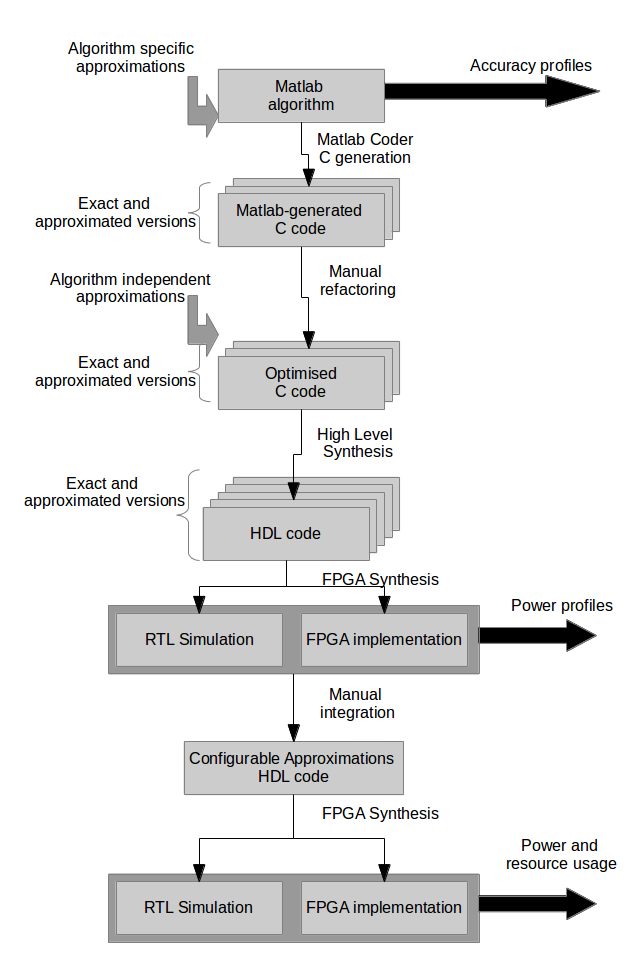
\includegraphics[width=0.9\columnwidth]{img/experimental_flow.png}
  \caption{Experimental design flow.}
  \label{fig:experimental_flow}
\end{figure}
